\section{GeoSPARQL}
\label{sec:GeoSPARQL}
%%%%%%%%%%%%%%%%%%%%%%%%%%%%%%%%%%%%%%%%%%%%%%%%%%%%%%%%
\begin{figure}[h!]
\begin{center}
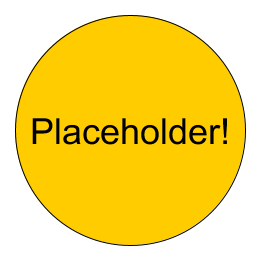
\includegraphics[width=.8\textwidth]{figures/placeholder}
\end{center}
\caption{Schema Diagram for the GeoSPARQL Pattern. The visual notation is explained in Chapter \ref{chap:prelims}.}
\label{fig:GeoSPARQL}
\end{figure}
\subsection{Summary}
\label{sum:GeoSPARQL}
%%%%%%%%%%%%%%%%%%%%%%%%%%%%
GeoSPARQL does not define a comprehensive vocabulary for representing spatial information. Instead GeoSPARQL defines a core set of classes, properties and datatypes that can be used to construct query patterns. Many useful extensions to this vocabulary are possible, and we intend for the Semantic Web and Geospatial communities to develop additional vocabularies for describing spatial information.

%%%%%%%%%%%%%%%%%%%%%%%%%%%%%%%%%%%%%%%%%%%%%%%%%%%%%%%%
\subsection{Axiomatization}
\label{axs:GeoSPARQL}
%%%%%%%%%%%%%%%%%%%%%%%%%%%%
\begin{align}
% General Axioms\top &\sqsubseteq \forall\textsf{place.Holder} \\ 
\exists\textsf{place.Holder} &\sqsubseteq \top 
% Domain and Range Restrictions\top &\sqsubseteq \forall\textsf{place.Holder} \\ 
\exists\textsf{place.Holder} &\sqsubseteq \top 
% Inverse Aliases (if any)placeholder &\equiv holderplace^- 
\end{align}

%%%%%%%%%%%%%%%%%%%%%%%%%%%%%%%%%%%%%%%%%%%%%%%%%%%%%%%%
\subsection{Explanations}
\label{exp:GeoSPARQL}
%%%%%%%%%%%%%%%%%%%%%%%%%%%%
\begin{enumerate}
\item temporary item
\end{enumerate}

%%%%%%%%%%%%%%%%%%%%%%%%%%%%%%%%%%%%%%%%%%%%%%%%%%%%%%%%
\subsection{Competency Questions}
\label{cqs:GeoSPARQL}
%%%%%%%%%%%%%%%%%%%%%%%%%%%%
\begin{enumerate}[CQ1.]
\item temporary item
\end{enumerate}

\newpage
%%%%%%%%%%%%%%%%%%%%%%%%%%%%%%%%%%%%%%%%%%%%%%%%%%%%%%%%
% End Section
%%%%%%%%%%%%%%%%%%%%%%%%%%%%%%%%%%%%%%%%%%%%%%%%%%%%%%%%
%%%%%%%%%%%%%%%%%%%%%%%%%%%%%%%%%%%%%%%%%%%%%%%%%%%%%%%%